\documentclass[11pt,a4paper]{ctexart}
%以下为所使用的宏包
\usepackage{ulem}%下划线
\usepackage{amsmath,amsfonts,amssymb,amsthm,amsbsy}%数学符号
\usepackage{graphicx}%插入图片
\usepackage{booktabs}%三线表
%\usepackage{indentfirst}%首行缩进
\usepackage{tikz}%作图
\usepackage{appendix}%附录
\usepackage{array}%多行公式/数组
\usepackage{makecell}%表格缩并
\usepackage{siunitx}%SI单位--\SI{number}{unit}
\usepackage{mathrsfs}%数学字体
\usepackage{enumitem}%列表间距
\usepackage{multirow}%列表横向合并单元格
\usepackage[colorlinks,linkcolor=red,anchorcolor=blue,citecolor=green]{hyperref}%超链接引用
\usepackage{float}%图片、表格位置排版
\usepackage{pict2e,keyval,fp,diagbox}%带有斜线的表格
\usepackage{fancyvrb,listings}%设置代码插入环境
\usepackage{minted}%代码环境设置
\usepackage{fontspec}%字体设置
\usepackage{color,xcolor}%颜色设置
\usepackage{titlesec} %自定义标题格式
\usepackage{tabularx}%列表扩展
\usepackage{authblk}%titlepage作者信息
\usepackage{nicematrix}%更好的矩阵标定
\usepackage{fbox}%更多浮动体盒子

\usepackage{tkz-graph}
\tikzset{
  LabelStyle/.style = { rectangle, rounded corners, draw,
                        minimum width = 2em,
                        text = red, font = \bfseries },
  VertexStyle/.append style = { inner sep=5pt,
                                font = \Large\bfseries},
  EdgeStyle/.append style = {->, bend left} }
%以下是页边距设置
\usepackage[left=0.5in,right=0.5in,top=0.81in,bottom=0.8in]{geometry}

%以下是段行设置
\linespread{1.4}%行距
\setlength{\parskip}{0.1\baselineskip}%段距
\setlength{\parindent}{2em}%缩进


%其他设置
\numberwithin{equation}{section}%公式按照章节编号
\newenvironment{point}{\raggedright$\blacktriangleright$}{}
\newenvironment{algorithm}[1]{\vspace{12pt} \hrule\hrule \vspace{3pt} \noindent\textbf{\color[HTML]{E63F00}Algorithm } \,\textit{#1} \vspace{3pt} \hrule\vspace{6pt}
}{\vspace{6pt}\hrule\hrule \vspace{12pt}} % 算法伪代码格式环境

%代码环境\lst设置
\definecolor{CodeBlue}{HTML}{268BD2}
\definecolor{CodeBlue2}{HTML}{0000CD}
\definecolor{CodeGreen}{HTML}{2AA1A2}
\definecolor{CodeRed}{HTML}{CB4B16}
\definecolor{CodeYellow}{HTML}{B58900}
\definecolor{CodePurPle}{HTML}{D33682}
\definecolor{CodeGreen2}{HTML}{859900}
\lstset{
    basicstyle=\tt,%字体设置
    numbers=left, %设置行号位置
    numberstyle=\tiny\color{black}, %设置行号大小
    keywordstyle=\color{black}, %设置关键字颜色
    stringstyle=\color{CodeRed}, %设置字符串颜色
    commentstyle=\color{CodeGreen}, %设置注释颜色
    frame=single, %设置边框格式
    escapeinside=`, %逃逸字符(1左面的键),用于显示中文
    %breaklines, %自动折行
    extendedchars=false, %解决代码跨页时,章节标题,页眉等汉字不显示的问题
    xleftmargin=2em,xrightmargin=2em, aboveskip=1em, %设置边距
    tabsize=4, %设置tab空格数
    showspaces=false, %不显示空格
    emph={TRUE,FALSE,NULL,NAN,NA,<-,},emphstyle=\color{CodeBlue2}, %其他高亮}
}


%节标题格式设置
\titleformat{\section}[block]{\large\bfseries}{Problem \arabic{section}}{1em}{}[]
\titleformat{\subsection}[block]{}{Question \arabic{section}.(\alph{subsection})}{1em}{}[]
% \titleformat{\subsubsection}[block]{\normalsize\bfseries}{    \arabic{subsection}-\alph{subsubsection}}{1em}{}[]
% \titleformat{\paragraph}[block]{\small\bfseries}{[\arabic{paragraph}]}{1em}{}[]


% \titleformat{\sectioncommand}[shape]{format}{title-label}{sep}{before-title}[after-title]


%SumatraPDF反向搜索命令行
%"C:\Users\彭拓锐Vincent\AppData\Local\Programs\Microsoft VS Code\Code.exe" "C:/Users/彭拓锐Vincent/AppData/Local/Programs/Microsoft VS Code\resources\app\out\cli.js" -r -g "%f:%l"

% 中文字号
% 初号42pt, 小初36pt, 一号26pt, 小一24pt, 二号22pt, 小二18pt, 三号16pt, 小三15pt, 四号14pt, 小四12pt, 五号10.5pt, 小五9pt

\begin{document}

\begin{center}\thispagestyle{plain}
    {\LARGE\textbf{Regression Analysis}}

    {\Large\textbf{2023 Fall HW1}}

    Tuorui Peng\footnote{TuoruiPeng2028@u.northwestern.edu} 
\end{center}

\thispagestyle{myheadings}\markright{Compiled using \LaTeX}

\pagestyle{myheadings}\markright{Tuorui Peng}

% Notation: Fourier transform is denoted $ \fallingdotseq $, say 
% \begin{align*}
%      g(t)\fallingdotseq G(\omega )
% \end{align*}
% (and inverse transform $ G(\omega )\risingdotseq g(t) $)



\section{}
The problem is solved with the following algorithm:
\begin{algorithm}{Solve $ Rx=b $ with $ R $ being upper-triangular}
    \textbf{Given:} $ R = \{r_{ij}\}_{0\leq i\leq j\leq n} \in \mathbb{R}^{n\times n}$ upper-triangular as stated, $ b\in \mathbb{R}^n $

    Initialize $ x_{n:(n+1)} = []$, for $ i=n:1 $

    \begin{enumerate}[topsep=2pt,itemsep=2pt]
        \item We already got $ \vec{x}_{n:(i+1)} $
        \item Focus on $ R_{i,:} $, we have
        \begin{align*}
            \sum_{j=i}^n r_{ij}x_j = b_i \Rightarrow x_i = \frac{b_i - \sum_{j=i+1}^n r_{ij}x_j}{r_{ii}}
        \end{align*}
        \item Solve $ x_{i} $ from $ x_{n:(i+1)} $, and now we have $ x_{n:i} $
    \end{enumerate}
    
    \textbf{Return:} $ x_{n:1}=x $
    
\end{algorithm}
    
\section{}

\subsection{}
Since we have $ m<n $ and $ A $ has full row rank, we have its right inverse matrix
\begin{align*}
    A_r := A^T(AA^T)^{-1} \in \mathbb{R}^{n\times m} 
\end{align*}
in this way $ \mathcal{S} $ could be represented as
\begin{align*}
    \mathcal{S} = \{x|x=A^T(AA^T)^{-1}b + \xi  ,\,\xi \in \mathrm{Null}(A)\} \subset \mathbb{R}^n
\end{align*}

and now the optimization problem is formulated as
\begin{align*}
    \pi_\mathcal{S}(y):=&\mathop{ \arg\min }\limits_{x\in\mathcal{S}} \left\Vert y-x \right\Vert ^2\\
    =& \mathop{ \arg\min }\limits_{\xi \in \mathrm{Null}(A)} \left\Vert y-A^T(AA^T)^{-1}b - \xi \right\Vert ^2\\
\end{align*}
into a constraint optimization problem, and the Lagrangian function is
\begin{align*}
    \mathcal{L}(\xi,\lambda) =& \left\Vert y-A^T(AA^T)^{-1}b - \xi \right\Vert ^2 + \lambda^TA\xi,\quad \lambda \in\mathbb{R}^m \\
     \Rightarrow& \begin{cases}
        y-A^T(AA^T)^{-1}b - \xi = A^T\lambda \\
        A\xi = 0
    \end{cases}\\
     \Rightarrow &Ay-b=AA^T\lambda  \Rightarrow \lambda = (AA^T)^{-1}(Ay-b)\\
    \Rightarrow &\xi =(I-A^T(AA^T)^{-1}A)y\\
    \Rightarrow &\pi_\mathcal{S}(y) = A^T(AA^T)^{-1}b + (I-A^T(AA^T)^{-1}A)y
\end{align*}

\subsection{}

\begin{figure}[H]
    \centering
    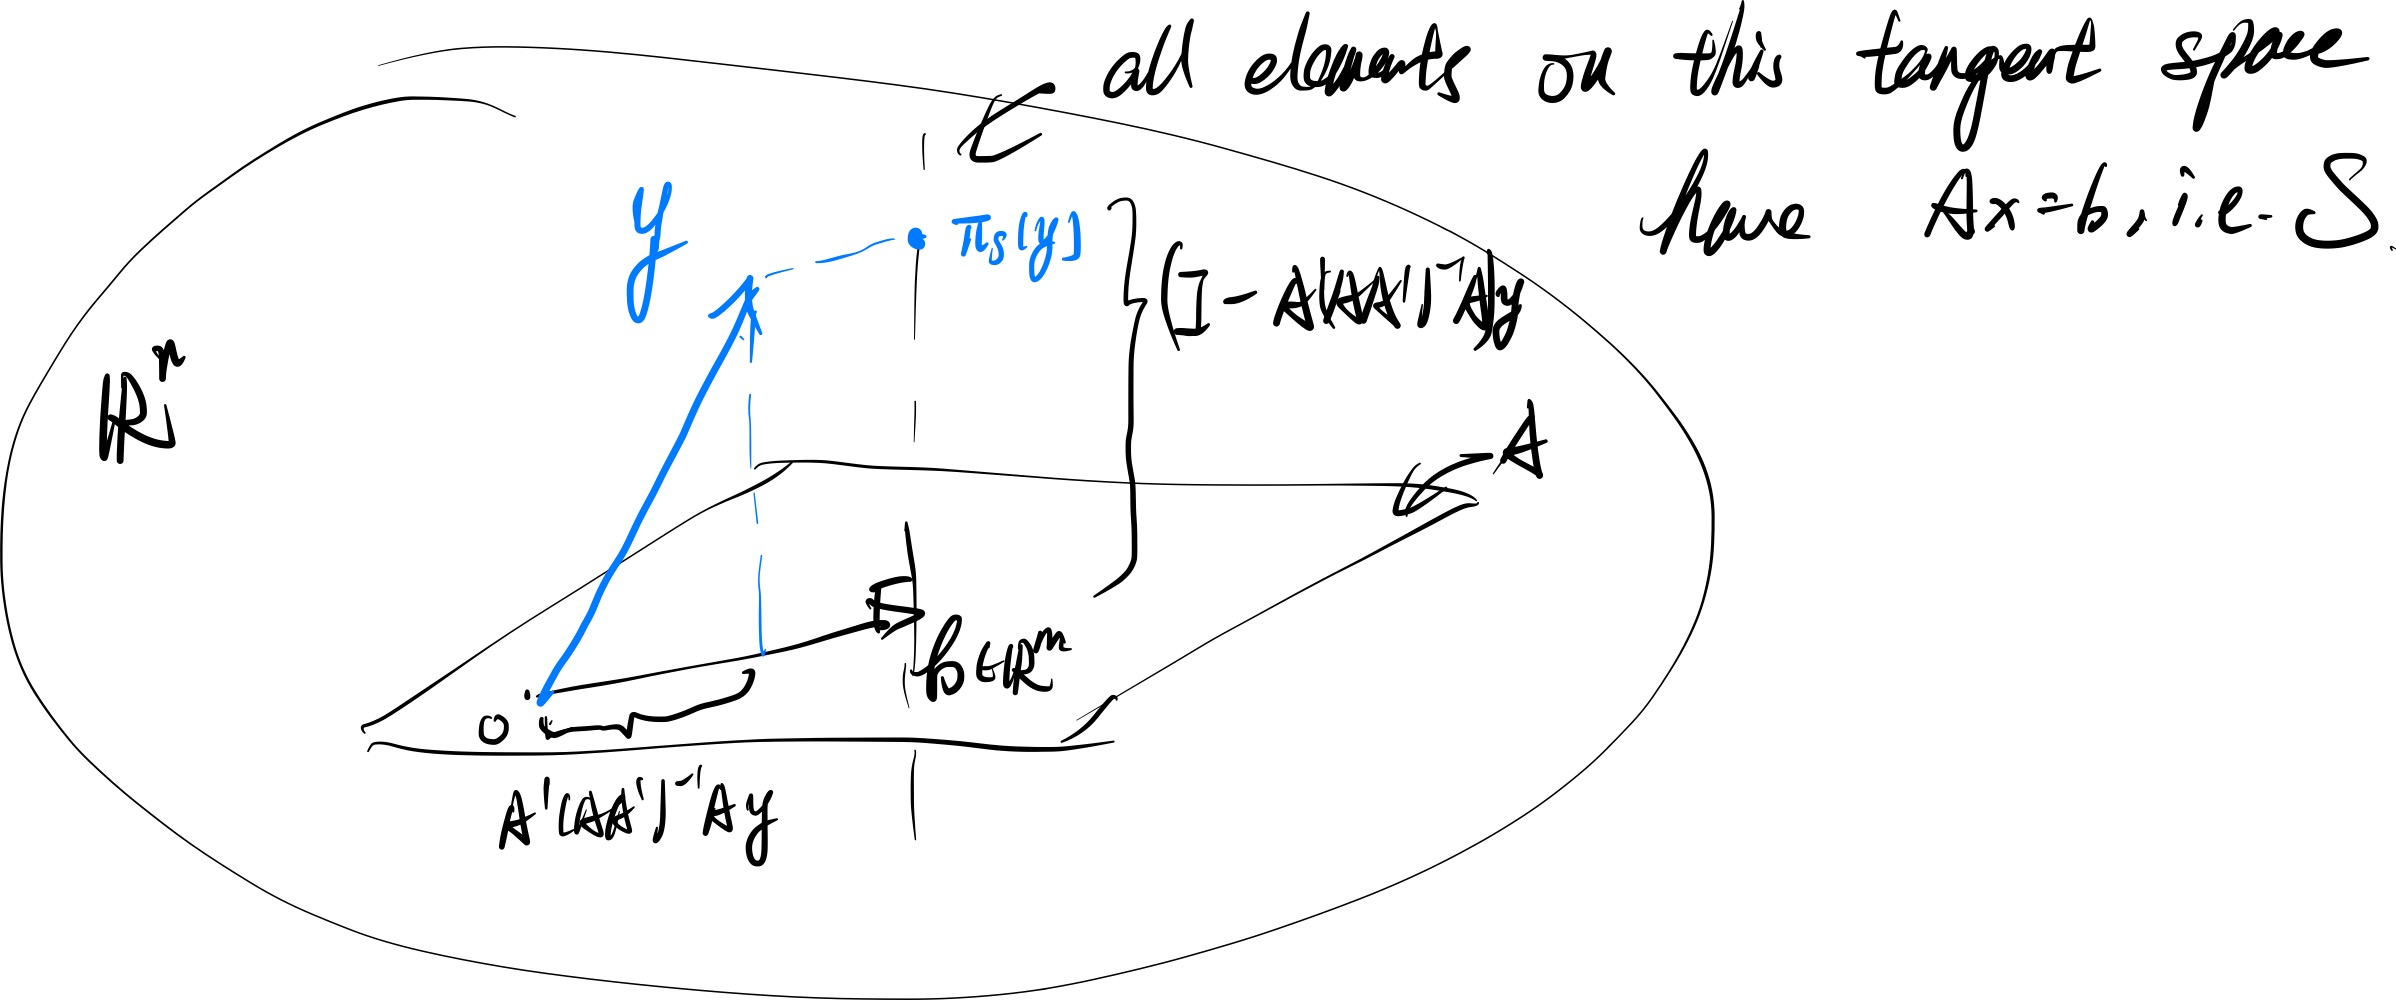
\includegraphics[width=0.7\linewidth]{HW1Pic1.jpg}
    \caption{Illustration of $ \pi_\mathcal{S}(y) $}
\end{figure}


\section{}

\subsection{}
Verify directly:
\begin{align*}
    &H_u'=(I-2uu')' = I-2uu' = H_u\\
    &H_u'H_u = (I-2uu')(I-2uu') = I-4uu'+4uu'u'u = I 
\end{align*}

\subsection{}
\begin{figure}[H]
    \centering
    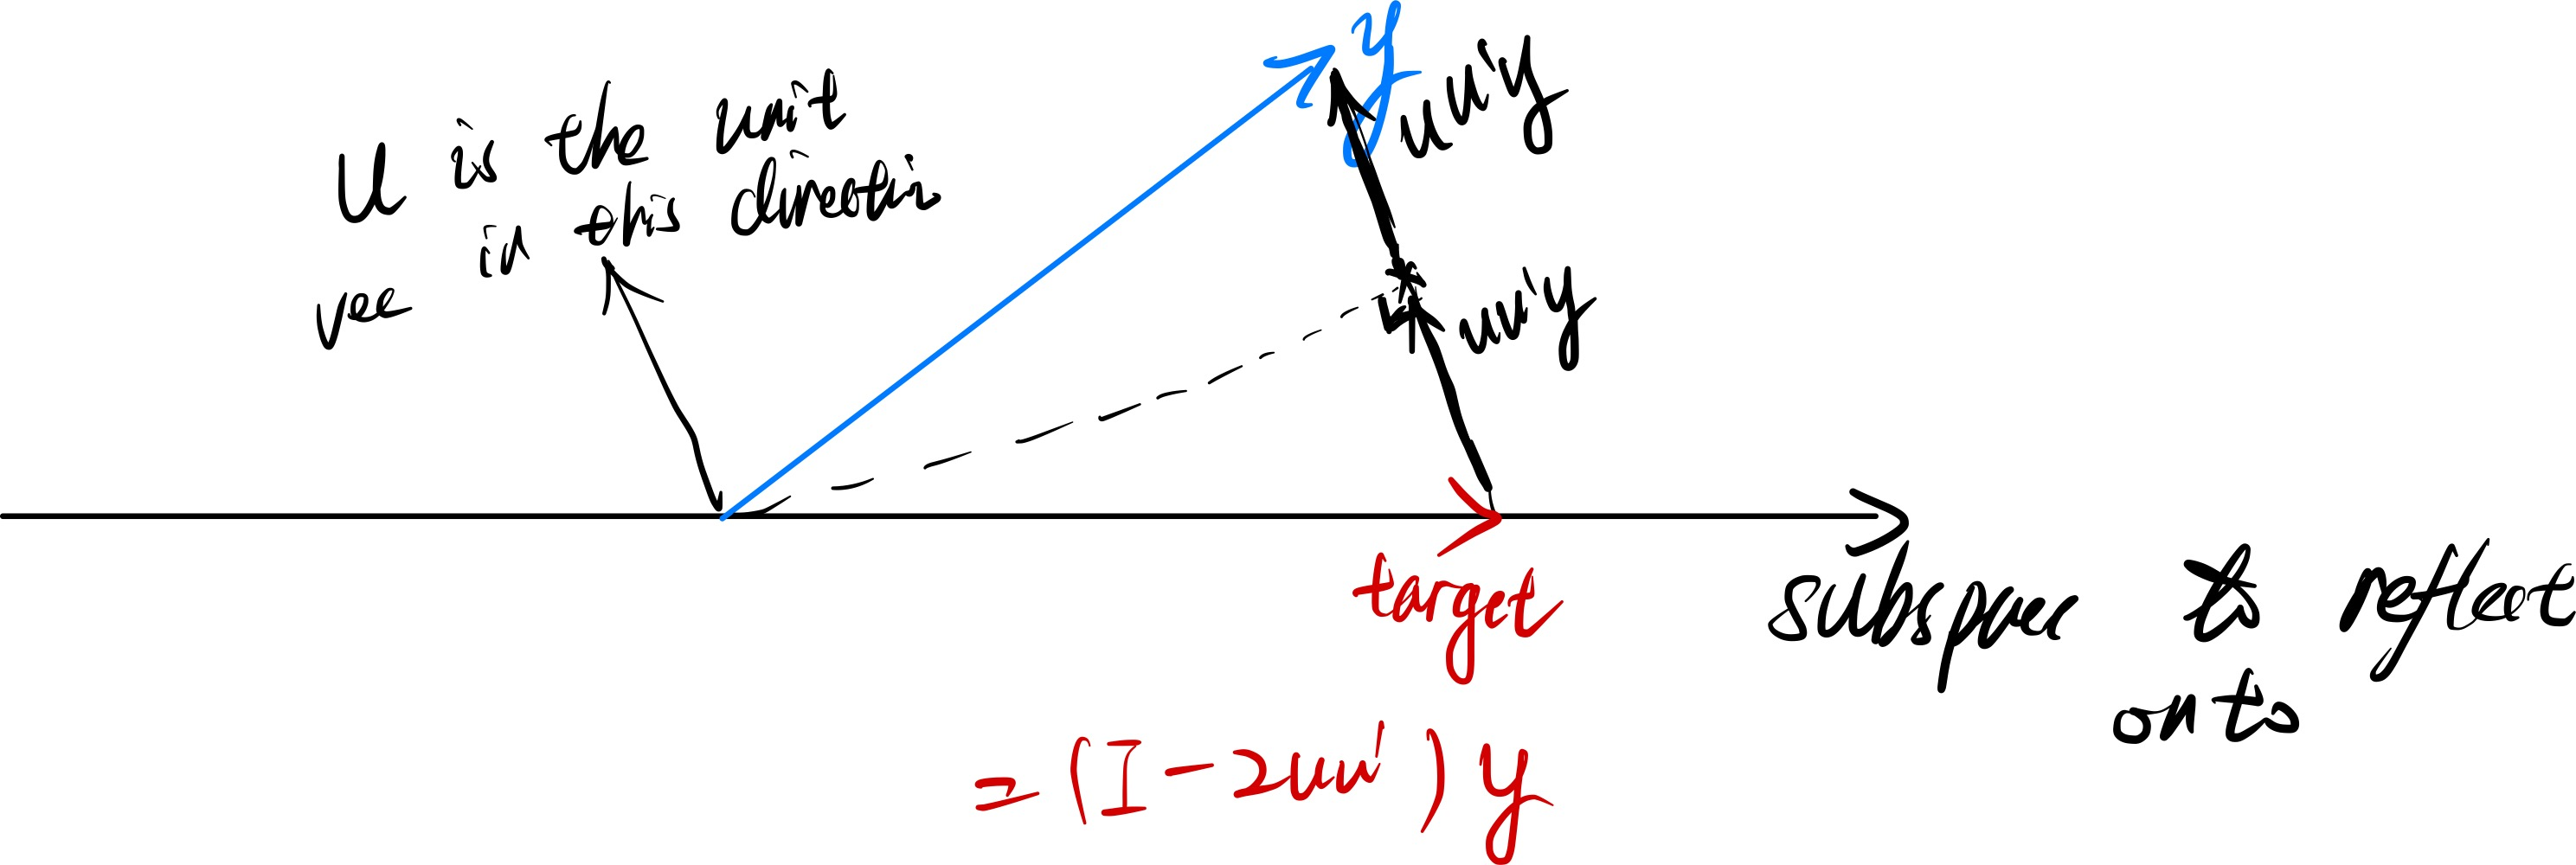
\includegraphics[width=0.7\linewidth]{HW1Pic2.jpg}
    \caption{Illustration of the reflection process}
\end{figure}


\subsection{}
So here $ e_1 $ is the `direction of subspace' we want to reflect onto. We can see that here $ v $ is just the angular bisector of $ \langle x,e_1\rangle $. Denote $ e_x = x/\left\Vert x \right\Vert $, the unit vector in $ x $ direction. Then we have
\begin{align*}
    H_vx=&\left( I-2\dfrac{ (e_x+e_1)(e_x+e_1)' }{ \left\Vert e_x+e_1 \right\Vert^2  }  \right) x\\
    =&\dfrac{ \left\Vert x \right\Vert  }{ \left\Vert e_x+e_1 \right\Vert^2 }\left( \left\Vert e_x+e_1 \right\Vert^2e_x-2(e_x+e_1)(e_x+e_1)'e_x \right)  \\
    =&\dfrac{ \left\Vert x \right\Vert  }{ \left\Vert e_x+e_1 \right\Vert^2 }\left((2+2e_x\cdot e_1)e_x-2(1+e_x\cdot e_1)(e_x+e_1) \right)\\
    =&\dfrac{ \left\Vert x \right\Vert  }{ 2+2e_x\cdot e_1 }\times -2(1+e_x\cdot e_1)e_1\\
    =&-\left\Vert x \right\Vert e_1
\end{align*}

\subsection{}
i.e. to prove that operator $ H $ is norm-preserving. We have
\begin{align*}
    \left\Vert Hx \right\Vert _2^2 =& x'H'Hx\\
    =& x'H_{u_k}'H_{u_{k-1}}'\cdots H_{u_1}'H_{u_1}\ldots H_{u_{k-1}}H_{u_k}x \\
    =& x'x = \left\Vert x \right\Vert _2^2 
\end{align*}

\subsection{}
as definition

\begin{align*}
    u = \dfrac{ a_1/\left\Vert a_1 \right\Vert +e_1 }{ \left\Vert a_1/\left\Vert a_1 \right\Vert +e_1 \right\Vert  } ,\qquad H_u = I-2uu'
\end{align*}

\subsection{}
Notation: the $ l^\mathrm{ th }  $ unit vector in $ \mathbb{R}^m $ is denoted $ e_{m,l} $. We have
\begin{align*}
    &\mathop{ u }\limits_{k+1}=\dfrac{ b_1/\left\Vert b_1 \right\Vert + e_{k+1,1}  }{ \left\Vert b_1/\left\Vert b_1 \right\Vert + e_{k+1,1} \right\Vert  },\quad F=I-2uu'\\
    &\text{Reflection: }S=\begin{bmatrix}
        \mathop{ I }\limits_{(n-k-1)\times (n-k-1)} & 0\\
        0& \mathop{ F }\limits_{(k+1)\times (k+1)} 
    \end{bmatrix}
\end{align*}

\subsection{}
Use the process in the previous subproblem, say it could reflect the $ i^\mathrm{ th }  $ column, denoted by $ S_i $. Then we could use 
\begin{align*}
    \Xi=S_{n-1}S_{n-2}\ldots S_1 
\end{align*}
to reflect all $ n $ columns. i.e.
\begin{align*}
    \Xi A = S_{n-1}S_{n-2}\ldots S_1  A = \text{upper triangular}
\end{align*}

we can write down the $ Q $ and $ R $
\begin{align*}
    A=QR,\quad Q=S_1S_2\ldots S_{n-1},\quad R=S_{n-1}S_{n-2}\ldots S_1  A
\end{align*}

\section{}
Notation: in this section I use $ v_i $ in place of $ s_i $, i.e. the eigenvector of $ A $. And further I use the convention that we have $ S $ is orthonormal (which can always be valid with some transform to $ \Lambda  $).
\subsection{}
To $ \mathrm{sgn}(v_1'x^0)\lambda _1v_1 $, i.e. $ \pm\lambda _1v_1 $.
\subsection{}
Note that in each step $ \dfrac{ 1 }{ \left\Vert x^k \right\Vert  }  $ just acts as a scalar. So doing $ n $ iteration with each step a scalar multiplication IS EQUIVALENT TO doing $ n $ iteration with only the last step a scalar (to unitary). So we could express a $ n+1 $ steps iteration as
\begin{align*}
    x^{n} = \xi A^{n}x^0 ,\quad x^{n+1}=\dfrac{ 1 }{ \left\Vert x^n \right\Vert  }Ax^n ,\quad \xi \in\mathbb{R}
\end{align*}
in which we denote the `un-scaled' $ A^nx^0 $ as $ \tilde{x}^n $, i.e. $ x^n=\xi \tilde{x}^n $. Then
\begin{align*}
    \tilde{x}^n= A^nx^0=(S\Lambda S^{-1})^nx^0 = S\Lambda^nS^{-1}x^0,\quad \forall n
\end{align*}

Then we have
\begin{align*}
    x^{n+1} = \dfrac{ 1 }{ \left\Vert S\Lambda ^{n}S^{-1} x^0 \right\Vert  } S\Lambda ^{n+1}S^{-1} x^0 
\end{align*}


in which spectrum of $ \dfrac{ 1 }{ \left\Vert S\Lambda ^{n}S^{-1} x^0 \right\Vert  } S\Lambda ^{n+1}S^{-1} $ is simply
\begin{align*}
    \dfrac{ 1  }{ \left\Vert S\Lambda ^{n}S^{-1} x^0 \right\Vert  } S\Lambda ^{n+1}S\mathop{ \sim = }\limits^{(i)} &\dfrac{ 1 }{ \left\Vert \Lambda ^{n}  \right\Vert  } S\Lambda ^{n+1}S =  S\mathrm{diag}\{\lambda _1, \lambda _2\left(\dfrac{ \lambda _2 }{ \lambda _1 }\right)^n,\ldots , \lambda _n\left(\dfrac{ \lambda _n }{ \lambda _1 }\right)^n \}S^{-1}\\
    \to & S\mathrm{diag}\{\lambda _1, 0,\ldots, 0\}S^{-1}=\lambda _1v_1v_1'
\end{align*}
in which $ (i) $ means only up to a constant $ \sim O(1) $

And finally
\begin{align*}
    x^{n+1}\to\propto&  \lambda _1v_1v_1'x^0\propto v_1\mathrm{sgn}(v_1'x^0)\\
    x^{n+2}\to& A\dfrac{ x^{n+1} }{ \left\Vert x ^{n+1}\right\Vert  }=Av_1\mathrm{sgn}(v_1'x^0)=\mathrm{sgn}(v_1'x^0)\lambda _1v_1 
\end{align*}

\section{}

\subsection{}
\begin{align*}
    \begin{cases}
        x = (A-BD^{-1}C)^{-1}(a-BD^{-1}b)\\
        y = (D-CA^{-1}B)^{-1}(b-CA^{-1}a)
    \end{cases} 
\end{align*}
\subsection{}
Using the above fomula, we have
\begin{align*}
    y =& (C^{-1}+V'A^{-1}U)^{-1}V'A^{-1}z \Rightarrow x=A^{-1}(z-Uy)=\left( A^{-1}-A^{-1}U(C^{-1}+V'A^{-1}U)^{-1}V'A^{-1}\right)z\\
     \Rightarrow & (A+UCV')^{-1}= A^{-1}-A^{-1}U(C^{-1}+V'A^{-1}U)^{-1}V'A^{-1}
\end{align*}

\section{}
\subsection{}
Prove it directly
\begin{align*}
     \mathrm{L.H.S.} = (a_2+(a_1-a_2))b_1+(a_1-(a_1-a_2))b_2=a_2b_1+a_1b_2+(a_1-a_2)(b_1-b_2)\geq a_2b_1+a_1b_2 = \mathrm{R.H.S.}
\end{align*}
\subsection{}
Denote $ P_{\mathrm{ swap }(i,j) } $ as the operator to swap the $ i^\mathrm{ th }  $ and $ j^\mathrm{ th }  $ element. 
\begin{enumerate}[topsep=2pt,itemsep=2pt]
    \item Since $ P_{\mathrm{ swap }(i,j) } $ keep all other $ n-2 $ elements unchanged, we can make use of the above 2-dimensional inequality, we have the following statement:  
    \begin{quote}
        If $ P_{\mathrm{ swap }(i,j) } $ is \textbf{moving the larger element to a higher larger index, then the inequality is preserved}. Say swapping $ v_n@ n \leftrightarrow v_{n-1}@ n-1 $ then the inequality perserve, while $ v_n@n-1 \leftrightarrow v_{n-1}@n $ does not.
    \end{quote}
    i.e.
    \begin{align*}
        u' \tilde{v}\geq u'P_{\mathrm{ swap }(i,j)}\tilde{v}\Leftrightarrow \tilde{v}_i\geq \tilde{v}_j \& i>j
    \end{align*}
    \item Then we prove that: any permutation matrix $ P\in\mathcal{P}_n $ could be represented as products of $ P_{\mathrm{ swap }(i,j) } $s, in which each $ P_{\mathrm{ swap }(i,j) } $ is moving the larger element to a higher larger index for the declared $ u,\tilde{v} $.
    
    We do it by the following iteration process:
    \begin{algorithm}{Decomposition $ Pv = \prod P_{\mathrm{ swap }(i,j) } v $ which perserce inequality}
        \textbf{For} $ \imath = n:1 $:
        \begin{itemize}[topsep=2pt,itemsep=2pt]
            \item Move $ v_k $ to the desired position as in $ Pv $ by repeatedly swap it with `the first element on its left with subscript smaller than itself'. e.g. to move $ v_{n-1} $ which is now at position $ n $ to position $ n-3 $, with $ v_{n} $ already at position $ n-2 $, i.e.
            \begin{align*}
                \ldots, v_{n-3}, v_n , v_{n-2}, v_{n-1}
            \end{align*}
            we do by following:
            \begin{align*}
                &\ldots, v_{n-3}, v_n , v_{n-1}, v_{n-2}\qquad \text{swap } v_{n-1} \text{ with } v_{n-2}\\
                &\ldots, v_{n-1}, v_n , v_{n-3}, v_{n-2}\qquad v_n \text{ is skipped, then swap } v_{n-1} \text{ with } v_{n-3}
            \end{align*}
        \end{itemize}
        Repeat the above operation, which preserve the inquality, until $ v_{n:1} $ are all at the right position to become $ Pv $.

        Now we have $ u'v\geq u'Pv $
            
    \end{algorithm}
\end{enumerate}

\subsection{}
According to the above algorithm, we know that $ u'v\geq u'Pv $, $ \forall P\in\mathcal{P}_n $. Then we have
\begin{align*}
    u'v = & u'(\sum_{l=1}^k\lambda _l)v \geq u'\sum_{l=1}^k\lambda _lP_l,\quad w.r.t. \lambda _l\geq 0,\sum_{l=1}^k\lambda _l=1 \\
    =&u'Sv,\quad \forall S\in\mathcal{S}_n
\end{align*}
And also $ I\in \mathcal{S} $, thus
\begin{align*}
    u'v = \mathop{ \max }\limits_{S\in\mathcal{S}_n}u'Sv  
\end{align*}


\section{}

\subsection{}
Say we denote the SVD of $ A $ as $ A=\tilde{U}\tilde{\Sigma }\tilde{V} $, then we have
\begin{align*}
     \mathrm{L.H.S.} = tr(AB)=tr(\tilde{U}\tilde{\Sigma }\tilde{V}) = tr(\tilde{\Sigma}\tilde{V}B\tilde{U}) 
\end{align*}
and here we can define $ \tilde{B}\leftarrow \tilde{V}B\tilde{U} $. And on the other hand, singular values of a matrix preserve under unitary transformation, thus
\begin{align*}
    \sigma(\tilde{B})=\sigma(\tilde{V}B\tilde{U})=\sigma (B)
\end{align*}
so vNti is now
\begin{align*}
    tr(\tilde{\Sigma } \tilde{B}) \leq \sum_{i=1}^n \sigma _i(\tilde{\Sigma })\sigma _i(\tilde{B}) =
\end{align*}

Now we can re-define $ B\leftarrow \tilde{B} $, and $ A\leftarrow\tilde{\Sigma } $. So its equivalent to prove
\begin{align*}
    tr(AB)\leq \sum_{i=1}^n\sigma _i(A)\sigma _i(B),\quad \text{with }A\text{ being diagonal}
\end{align*}

\subsection{}

\begin{align*}
    tr(AB)= tr(AU\Sigma V') = tr(V'AU\Sigma ) = \sum_{i=1}^n \sigma _i v_i'Au_i = \sum_{i,j\leq n}\sigma _iv_{ij}a_{j}u_{ij}
\end{align*}
\subsection{}
Using $ xy\leq \dfrac{ 1 }{ 2 }(x^2+y^2)   $, we have
\begin{align*}
    tr(AB) =  \sum_{i,j\leq n}\sigma _iv_{ij}a_{j}u_{ij} \leq \dfrac{ 1 }{ 2 } \sum_{i,j\leq n}\sigma _i a_j(v_{ij}^2+u_{ij}^2)
\end{align*}

\subsection{}
Since $ U $ and $ V $ are both orthonormal bases, we have
\begin{align*}
    \sum_{j=1}^n v_{ij}v_{kj} = \delta _{ik},\quad \sum_{j=1}^n u_{ij}u_{kj} = \delta _{ik}
\end{align*}
so matrix $ \{v_{ij}^2\}_{i,j=1}^n $ has row sum $ 1 $ \& column sum $ 1 $ (similar for $ \{u_{ij}^2\}_{i,j=1}^n $). Then using notation in the previous problem, in which $ \mathcal{S}_n $ is the doubly stochastic matrices, we have
\begin{align*}
    \{v_{ij}^2\}_{i,j=1}^n, \{u_{ij}^2\}_{i,j=1}^n \in \mathcal{S}_n \Rightarrow \{\dfrac{ 1 }{ 2 }(v_{ij}^2+u_{ij}^2)\}\in \mathcal{S}_n
\end{align*}
then using the inequality $     \tilde{u}'\tilde{v} = \mathop{ \max }\limits_{S\in\mathcal{S}_n}\tilde{u}'S\tilde{v}   $, we can place $ \sigma _i(A), \sigma _i(B) $ as the $ \tilde{u},\tilde{v} $, respectively, and then we have
\begin{align*}
    tr(AB) \leq & \sum_{i,j\leq n}\sigma _i  \dfrac{ 1 }{ 2 } (v_{ij}^2+u_{ij}^2) a_j\\
    \leq &\sum_{i=1}^n \sigma _i(B)\sigma _i(A)
\end{align*}




\end{document}








    






























\end{document}